\chapter{Transfer Learning}
\label{ch:lesson38}

Training a good CNN from scratch (Chapters~\ref{ch:lesson34}--\ref{ch:lesson35}) took hundreds of labeled examples even for a toy task. Real target tasks are often data-starved: a handful of labeled medical scans, a new product category with 20 photos. \textbf{Transfer learning} sidesteps this by reusing a network already trained on a \emph{different}, data-rich task, on the theory that early-layer features (edges, blobs, simple textures) are useful for almost any visual task, not just the one they were originally trained on. This chapter demonstrates it on real photos, using a CIFAR-10 subset (\citelink{krizhevsky2009cifar}{Krizhevsky, 2009}).

\section{Source task and target task}

Set up two related but distinct tasks, both from CIFAR-10. The \textbf{source task} has plenty of data: distinguishing airplanes from automobiles, 300 training images each. The \textbf{target task} is the one we actually care about, and it's deliberately starved: distinguishing cats from trucks --- two classes the source task never saw at all --- with only \textbf{15 training images per class} (Figure~\ref{fig:l38-1}).

\begin{figure}[h]
\centering
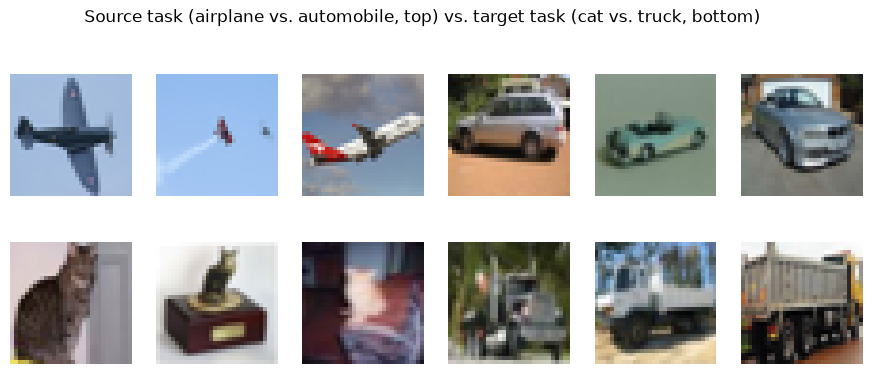
\includegraphics[width=0.9\textwidth]{figures/lesson38_fig01.png}
\caption{Sample target-task images: cats (top row) and trucks (bottom row).}
\label{fig:l38-1}
\end{figure}

\section{Three strategies}

\begin{enumerate}
  \item \textbf{From scratch} --- train a fresh CNN on only the 30 target images. This is the baseline: no transfer at all.
  \item \textbf{Frozen backbone (feature extraction)} --- pretrain a CNN backbone on the source task, then freeze its weights entirely and train only a new linear classifier on top of the features it produces for target images.
  \item \textbf{Fine-tuning} --- start from the same pretrained backbone, but keep updating it on the target data too, using a \emph{much smaller} learning rate for the backbone than for the new classifier head (the backbone already encodes useful structure; large updates from just 30 examples would wreck it).
\end{enumerate}

\begin{lstlisting}
def train_target(backbone, freeze_backbone, seed, epochs=200, lr=0.01, backbone_lr=None):
    model = Classifier(backbone, freeze_backbone)
    if freeze_backbone:
        opt = torch.optim.Adam(model.fc.parameters(), lr=lr)
    elif backbone_lr is not None:
        opt = torch.optim.Adam([
            {'params': model.backbone.parameters(), 'lr': backbone_lr},
            {'params': model.fc.parameters(), 'lr': lr},
        ])
    else:
        opt = torch.optim.Adam(model.parameters(), lr=lr)
\end{lstlisting}

Pretraining a small CNN backbone once on the source task, then evaluating all three strategies on the target task, averaged over 8 random seeds:

\begin{center}
\renewcommand{\arraystretch}{1.3}
\begin{tabular}{lrr}
\hline
\textbf{strategy} & \textbf{mean test acc} & \textbf{std} \\
\hline
from scratch    & 63.6\% & 6.8\% \\
frozen backbone & 69.5\% & 1.0\% \\
fine-tuned      & 76.7\% & 1.2\% \\
\hline
\end{tabular}
\end{center}

Both transfer strategies clearly beat training from scratch, and they're also dramatically more \emph{consistent} (lower standard deviation). Even though the source task never saw a cat or a truck, it learned generic low-level features (edges, color blobs, textures) that transferred to the new task.

Note that fine-tuning used a learning rate for the backbone roughly $30\times$ smaller than the classifier head's. With just 30 target examples, a larger backbone update would overfit those 30 images, discarding everything useful it had learned from the 600-image source task. This is the same catastrophic-forgetting failure mode as Chapter~\ref{ch:lesson35}'s overfitting curve, just applied to a network that started out already knowing something.

\section{In practice: pretrained backbones in one line}

The toy backbone above is trained from scratch on a toy task for illustrative purposes, but real transfer learning leverages existing networks available for reuse. \code{torchvision} ships architectures already pretrained on the full ImageNet dataset (Chapter~\ref{ch:lesson37}) --- 1.2 million images across 1,000 classes. Loading such a network, ready to use as a frozen feature extractor, is a single line of code:

\begin{lstlisting}
resnet = torchvision.models.resnet18(weights=torchvision.models.ResNet18_Weights.IMAGENET1K_V1)
resnet.fc = nn.Identity()  # strip the original 1000-class ImageNet head, keep the 512-d features
resnet.eval()
for p in resnet.parameters():
    p.requires_grad = False  # frozen, feature-extraction style
\end{lstlisting}

Total ResNet-18 parameters: $11{,}689{,}512$, all pretrained on ImageNet, none of them touched here.

ResNet-18 was trained on $224\times224$ images normalized by ImageNet's per-channel mean and standard deviation --- not the plain $[0,1]$ pixel scaling used everywhere else in this chapter --- so the target images need to be resized and renormalized before going through it. Extracting a 512-dimensional feature vector for every target image once (the backbone is frozen, so this only needs to happen once, not on every training step), then training a small linear head on top --- exactly the frozen-backbone strategy above, just with a very different backbone --- reaches $98.1\%\pm0.2\%$ mean test accuracy over 8 seeds, versus $69.5\%$ for the toy frozen backbone above.

Frozen ImageNet features push accuracy well past either toy strategy above, using nothing but a new linear layer trained on the same 30 target images --- no backbone training at all.

\textbf{A caveat on this comparison:} some of that gap is an unfair advantage, not just richer pretraining. ImageNet's 1,000 classes already include photos of cats and several vehicle types, unlike the toy source task, which only saw airplanes and automobiles --- so this isn't a perfectly controlled comparison of ``big general pretraining'' versus ``tiny 2-class pretraining'' in isolation; part of ResNet-18's edge comes from having directly seen the target classes during pretraining.

Nevertheless, the qualitative point holds, and it's the actual reason ImageNet-pretrained backbones are the default starting point in practice: a network trained on 1.2 million images learns far richer, more broadly transferable features than one trained on a couple thousand images of two categories ever could --- which is exactly what Chapter~\ref{ch:lesson37}'s architectures, and the vastly larger datasets they were trained on, are built to produce.

\subsection*{Exercises}
\begin{enumerate}
  \item Try \code{backbone\_lr=0.01} (i.e.\ no learning-rate difference between backbone and head) in the fine-tuning call. Does fine-tuned accuracy get better or worse, and does that match the catastrophic-forgetting explanation above?
  \item Try freezing \emph{most} of the backbone but fine-tuning only its last conv layer. Where does that land relative to fully-frozen and fully-fine-tuned?
  \item Swap the target task's classes from cat/truck to dog/automobile --- a target pair that overlaps the source task's \emph{domain} (vehicles) even more closely than cat/truck did. Does frozen-backbone accuracy improve further, and does that match the intuition that transfer works best when source and target share more underlying visual structure?
  \item Try unfreezing just ResNet-18's last residual stage (\code{resnet.layer4}) and fine-tuning it on the 30 target images at a small learning rate, the same way the toy backbone was fine-tuned above. Does it beat the fully-frozen ResNet-18 result, or is 30 images too few to safely update even a small fraction of 11 million parameters?
\end{enumerate}

\vfill
\fullcode{lesson38}{lesson38_transfer_learning}
